\chapter{Simulation der Ionenoptik}
\label{chap:Simulation}
Eine Simulation der Ionenoptik des Massenspektrometers ist sinvoll, um die Messergebnisse zu überprüfen, die Genauigkeit des Massenspektrometers zu bestimmen und Optimierungsansätze herrauszuarbeiten. Dafür wird das Programm \textit{SIMION} genutzt, das die Bewegung von geladenen Teilchen in elektrischen und magnetischen Feldern simulieren kann. Im Vergleich zu anderen Programmen ist \textit{SIMION} besonders geeignet, da es auf Ionen- und Elektronenoptik spezialisiert ist und die Möglichkeit bietet, die Simulationen mit geringem Aufwand mit eigenen Programmen zu erweitern. Im Folgenden soll die Methodik der Simulation und die Limitationen erläutert werden und im Anschluss die Ergebnisse der Simulationen präsentiert werden.

\section{\textit{SIMION}: Methodik und Limitation}
Zugrunde der Simulationen liegt bei \textit{SIMION} die numerische Lösung der Laplace-Gleichung (\ref{eq:laplace}) für das elektrische Potential $\Phi$ in einem gegebenen Raum \cite{SIMION}.
\begin{equation}
    \label{eq:laplace}
    \nabla^2 \Phi = 0.
\end{equation}
Um diese partielle Differentialgleichung zu lösen, nutzt das Programm finite Differenzverfahren (FDM), mit denen eine Ableitung über die Differenz zweier benachbarter Punkte approximiert wird. Dafür muss der Raum diskretisiert, also in ein Gitter aus Punkten aufgeteilt werden. Dabei ist es möglich mehrere Gitter mit verschiedenen Auflösungen zu definieren und diese innerhalb einer Simulation zu nutzen. Damit die iterative Lösung der Laplace-Gleichung schnell konvergiert, wird Überrelaxation (engl. \textit{Optimized Over-Relaxation, OOR}) verwendet. Statt bei jeder Iteration exakt nach der FDM zu aktualisieren, wird eine gewichtete Mischung aus der neuen und alten Lösung genommen. Um das Potential eines Gitters in jedem Punkt errechnen zu können, werden als Randbedingungen vom Nutzer definierte Elektroden und die Ränder der Simulation verwendet. Unterschieden wird dabei zwischen Dirichlet- und Neumann-Randbedingungen:
\begin{itemize}
    \item {Dirichlet-Randbedingungen:} Das Potential an der Elektrode ist auf einen vom Nutzer angegebenen Wert festgelegt.
    \item {Neumann-Randbedingungen:} Die Ableitung des Potentials entlang der normalen Richtung zum Rand fest wird festgelegt. In \textit{SIMION} wird $\frac{\partial \Phi}{\partial n} = 0$ gesetzt, was bedeutet, dass das elektrische Feld am Rand keine normale Komponente hat.
\end{itemize}

Aufgrund der Neumann-Randbedingungen „spiegelt“ sich das Feld an der Grenze. Dadurch verhält es sich so, als ob der Simulationsbereich künstlich erweitert würde, ohne dass sich Ladungen oder Potentiale jenseits des Rands befinden. Dies verhindert abrupte Feldänderungen an der Grenze und sorgt dafür, dass das Feld innerhalb des Simulationsbereichs realistisch bleibt. Das elektrische Feld $E$ kann dann mit dem errechneten Potential an jedem Ort bestimmt werden, um die Beschleunigung der Lorentzkraft auf geladene Teilchen zu ermitteln. Für die Iteration der Trajektorien wird eine Runge-Kutta-Verfahren 4. Ordnung angewandt. Die zeitliche Schrittweite ist dabei variabel. In einer Simulation werden vom Nutzer definierte Teilchen nach einander in das Feld gesetzt und ihre Trajektorie berechnet. 

Limitierend ist allgemein, dass die Teilchen dabei selbst nicht das Potential beeinflussen. Das bedeutet, dass sie auch nicht miteinander wechselwirken können und keine Raumladungseffekte berücksichtigt werden. Da innheralb dieser Arbeit aber unter Einzelstoßbedinungen gearbeitet wird, ist das nicht relevant. Angenommen wird auch, dass die Felder statisch sind und somit werden zeitabhängige Effekte, wie dem Induktionsgesetz, nicht berücksichtigt. Es ist aber trotzdem möglich die Felder in Abhängigkeit der Zeit mit eigener Programmierung zu verändern.

\section{Modellierung und Konfiguration}
Um die Ionenoptik der derzeit verwendeten Geometrie zu untersuchen, muss dieser akkurat modelliert werden. Anhand der originalen Designdateien des Plattenkondensators konnte eine vereinfachte Geometrie in \textit{SIMION} erstellt werden. Die Elektroden wurden zweidimensional modelliert und dann mit Zylindersymmetrie auf 3D erweitert. Abbildung \ref{fig:model} zeigt das Modell des Massenspektrometers in \textit{SIMION}. Zunächst wurden die derzeitigen Maße der Anlage eingesetzt, anhand der Simulation soll aber der Abstand des Detektors variiert werden.

\begin{figure}
    \centering
    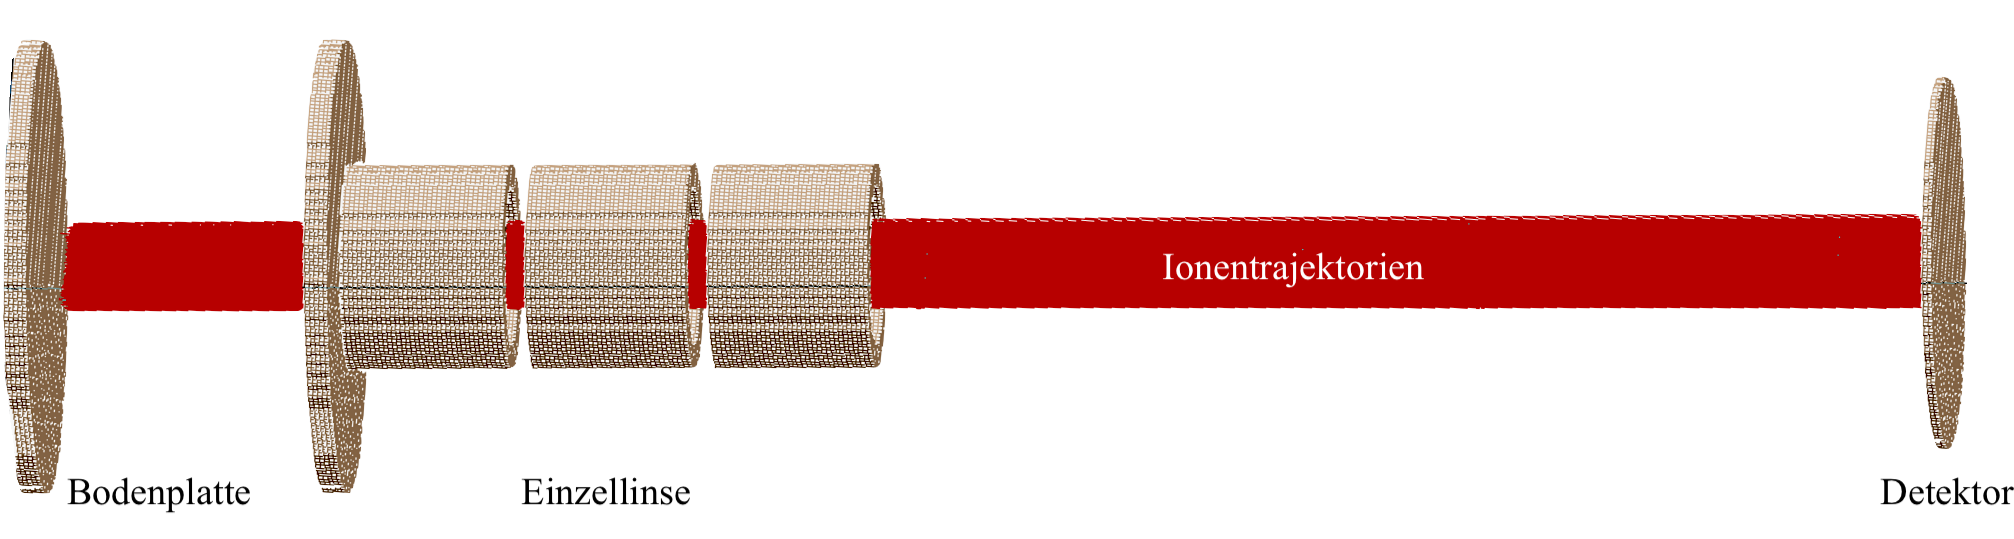
\includegraphics[width=1\textwidth]{Model.png}
    \caption[Modell des Massenspektrometers in \textit{SIMION}]{Modell des Massenspektrometers in \textit{SIMION}. Die Elektroden sind in Beige dargestellt, die Flugbahnen der Ionen in Rot. Dargestellt ist die Geometrie einer Flugstrecke von 410 mm.}
    \label{fig:model}
\end{figure}

Auf der Bodenplatte (in der Simulation links) wird ein positives Potential von mehreren Kilovolt angelegt, während die Deckenplatte und Einzellinse auf Masse (0 V) liegt. Genauso wie im Experiment wird die Linse vorerst nicht verwendet. Der Detektor (in der Simulation rechts) bekommt ein Potential von -2500 V, ähnlich dem in der Anlage. 

\subsection{Initialisierung der Ionen}
Die Interaktion der Elektronen mit dem Neutralgas wird in der Simulation nicht berücksichtigt. Stattdessen werden die Ionen im Pfad des Elektronenstrahls erschaffen, also in einem Streifen paralell zu den Platten. Um die räumliche Ausdehnung des Strahls zu berücksichtigen und, wie auch im Experiment zu beobachten, eine Verteilung der Flugstrecken der Ionen zu erhalten, wird das in der Auswertung des Strahlprofils bestimmte Profil des Elektronenstrahls genutzt. Die Ionen werden dann mit einer FWHM von $1.95$ mm um die Linie des Strahls gauß-verteilt. Da das Experiment von der Einzelstoßbedingung ausgeht, kann ein Ion nach dem Anderen simuliert werden und die Wechselwirkung zwischen Ionen vernachlässigt werden.

Die Art der Teilchen, so wie ihre Häufigkeitsverteilung können mit einem \textit{.fly2}-File definiert werden. Auch die räumliche Verteilung des Strahls wurde hierüber implementiert. Die verwendete Datei ist im Anhang \ref{fly2} zu finden. Für die kinetische Energie der Teilchen wird aufgrund der thermischen Bewegung angenommen. Dieser Wert ergibt sich, wenn man eine Maxwell-Boltzmann-Verteilung für die kinetische 
Energie der Ionen annimmt und die Temperatur der Ionen auf 300 K (Raumtemperatur) setzt: 
\begin{equation}
    \label{eq:kin}
    \left< E_{\text{kin}} \right> = \frac{3}{2} k_B T_{Raum} \approx \frac{1}{25} \text{ eV}.
\end{equation}

\subsection{Extraktion der Ionen}
Die Extraktion der Ionen erfolgt durch die Anlegung eines elektrischen Feldes zwischen den Platten, wie im Experiment. Damit der Vergleich so präzise wie möglich ist, wird das Potential auf der Bodenplatte zeitabhängig verändert. Dabei wird die Spannung von 0 auf 5000 V mit einer linearen Rampe in 50 ns erhöht, nachdem die Extraktionsverzögerung abgewartet wurde. Die Zeitabhängigkeit wurde dem Signalverlauf (dargestellt in \ref{fig:Signal}) entnommen. Die Ionen werden dann in einem Zeitfenster von 4 $\mu s$ extrahiert. Um das zeitabhängige Potential umzusetzen, wird ein \textit{Workbench}-File genutzt, das die Spannung in Abhängigkeit der Zeit definiert. In \textit{SIMION} können Potentiale angepasst werden, ohne das gesamte Potential-Array neu berechnen zu müssen. Dies ist möglich, da die Potentiale durch eine Überlagerung von Spannungen auf bereits existierenden Elektroden definiert sind.

\section{Vergleich der Simulation mit dem Experiment}
Um dieselben Informationen aus der Simulation zu gewinnen, wie sie auch im Experiment vom Detektor aufgenommen werden, werden Flugzeit und Position jedes Teilchens zum Auftreffpunkt aufgezeichnet. Diese können dann mit denselben Methoden wie die experimentellen Daten ausgewertet werden. Im Folgenden werden verschiedene Simulationen durchgeführt, um die Ionenoptik zu untersuchen. Dafür sollen zunächst die Ergebnisse aus dem Experiment nachsimuliert werden, um die Genauigkeit der Simulation zu überprüfen. 


\begin{figure}
    \centering
    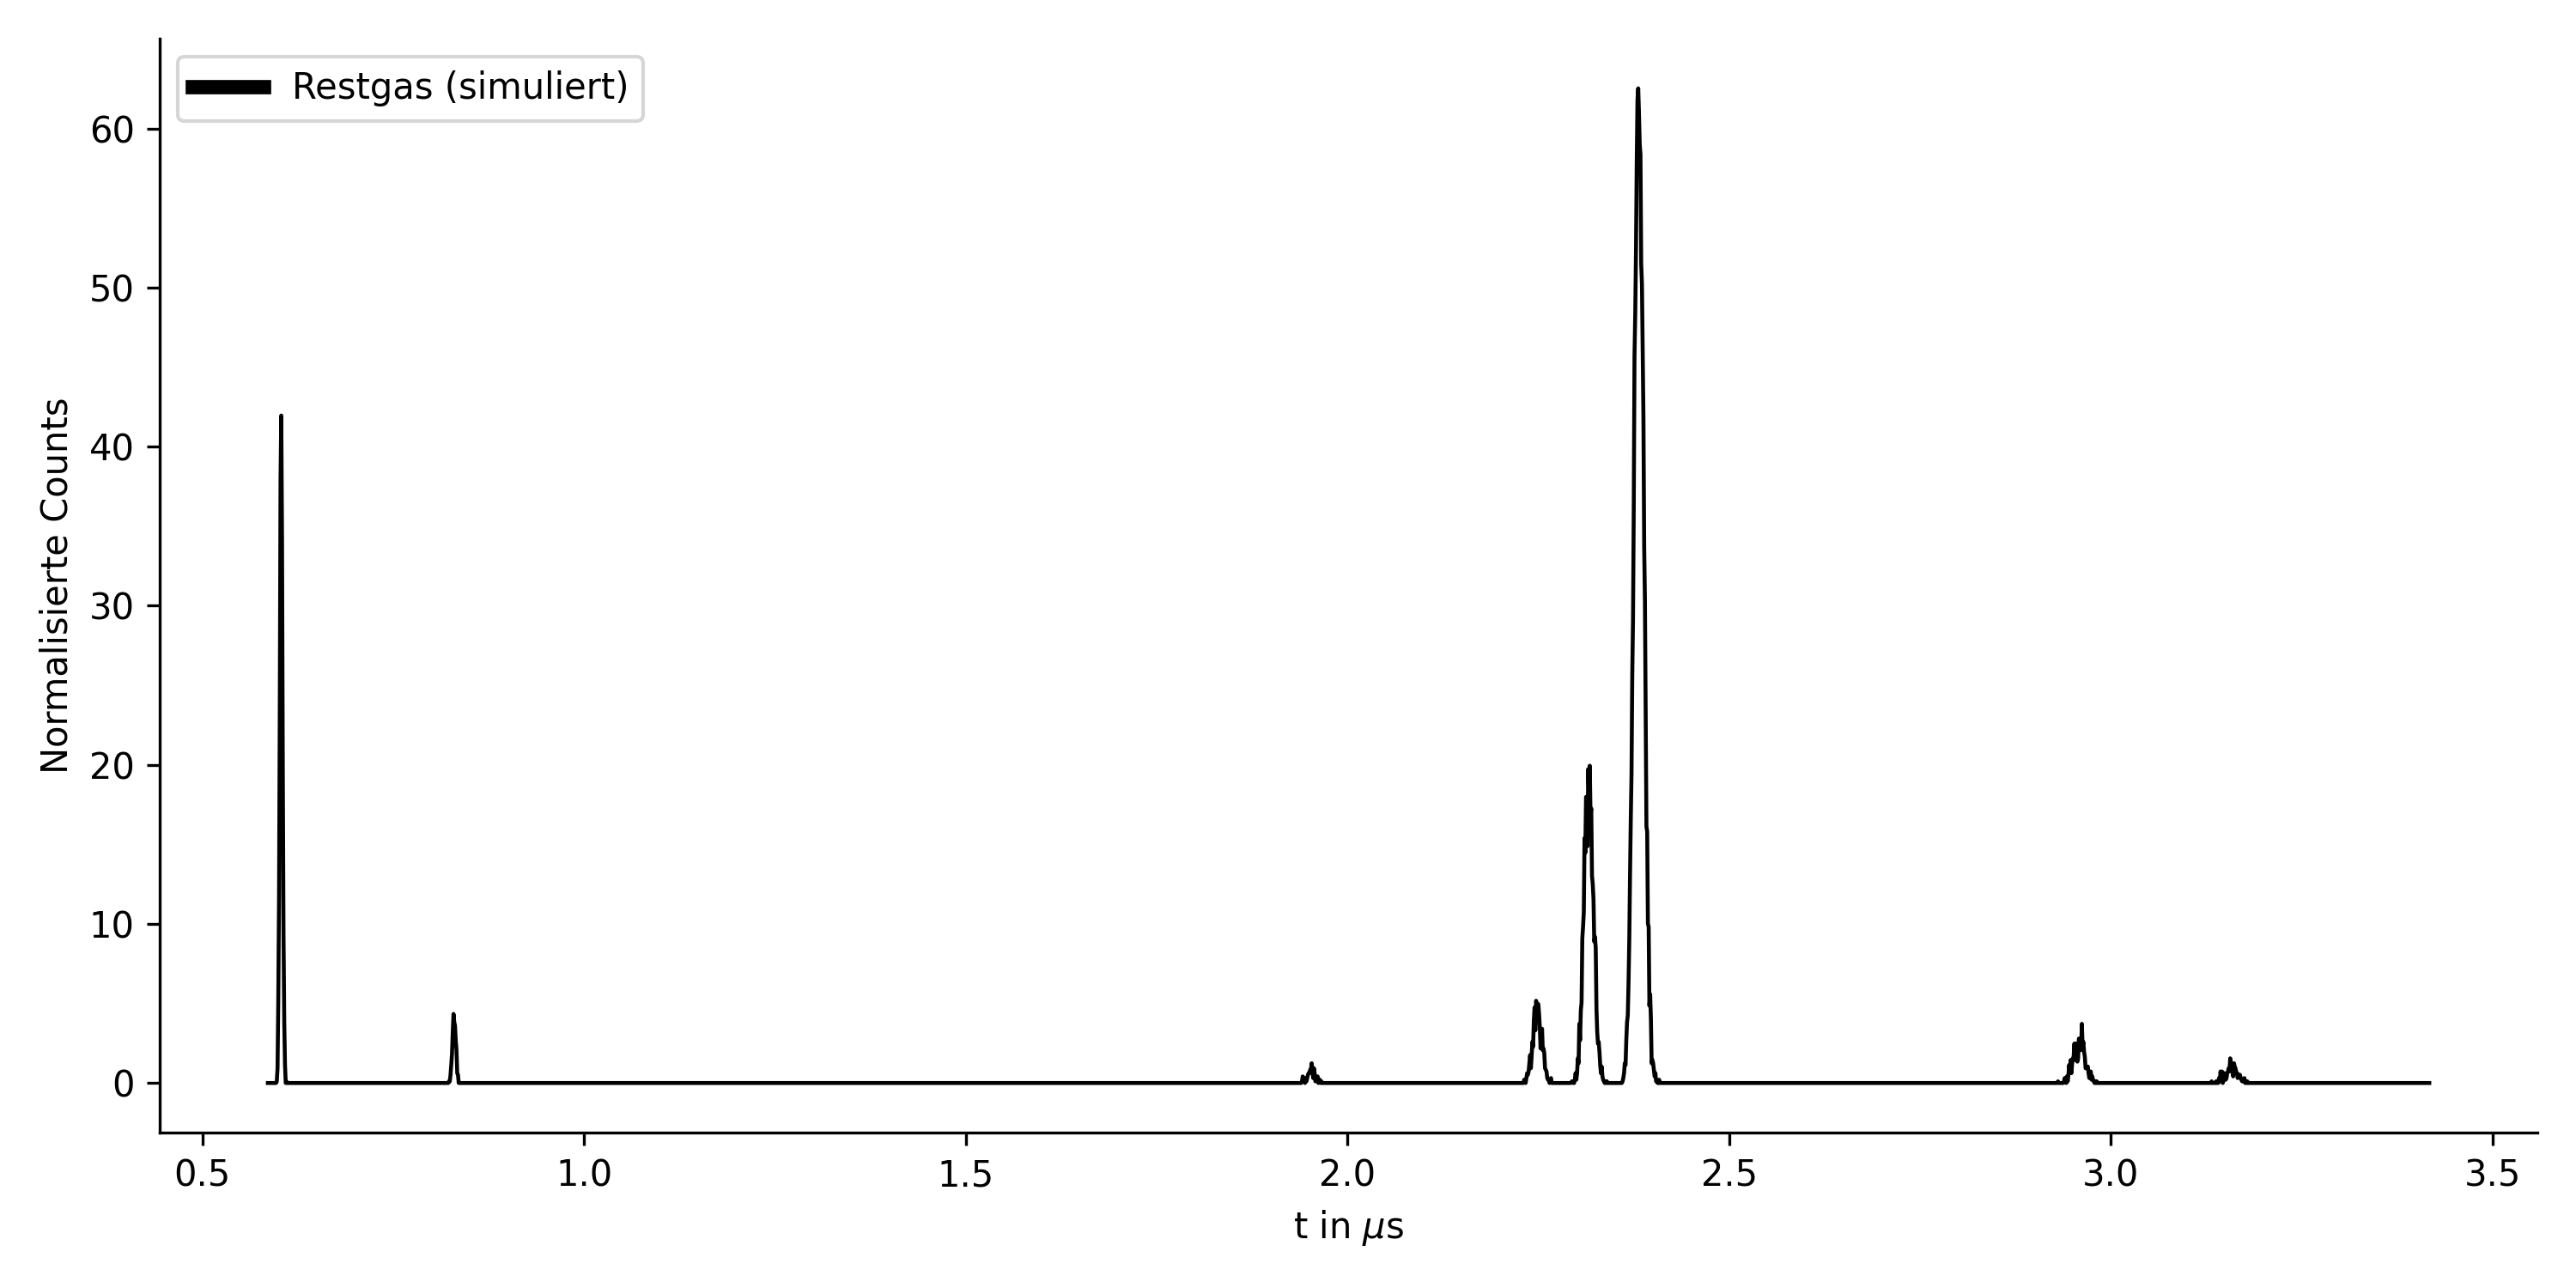
\includegraphics[width=.8\textwidth]{Restgas_Sim.png}
    \caption[Simuliertes Restgasspektrum]{Ein simuliertes Restgasspektrum, die Ionenverteilung wurde anhand der Auswertung des Restgasspektrums gesetzt.}
    \label{fig:Restgas_Sim}
\end{figure}

Implementiert man einen Ionenverteilung ähnlich der in der Auswertung des Restgasspektrums bestimmten, kann man ein vergleichbares Flugzeitspektrum aus simulierten Daten generieren. Abbildung \ref{fig:Restgas_Sim} zeigt ein solches Ergebnis. Die Flugzeitverteilung der Ionen ist ähnlich der im Experiment beobachteten. Die zeitliche Abweichung der simulierten Peaks zu den echten Daten beträgt weniger als 100 ns und kommt wahrscheinlich durch die vereinfachte lineare Umsetzung der kapazitiven Beschleunigungsplatte zustande. In der Simulation wird bestätigt, dass die Ionen in einem Zeitfenster von 4 $\mu s$ extrahiert werden. Die Peaks sind schärfer als im Experiment und es ist deutlich weniger Rauschen vorhanden. Das liegt daran, dass die Simulation keine Störeffekte berücksichtigt und der Detektor idealisiert ist. Dass das Ergebnis kein Linienspektrum ist, liegt daran, dass der Strahl als räumlich ausgedehnt simuliert wird.

\begin{figure}[H]
    \centering
    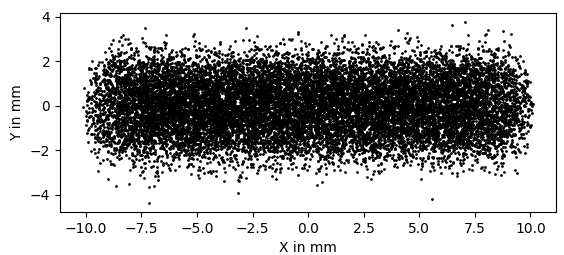
\includegraphics[width=.65\textwidth]{Sim_Positions_Scatter.png}
    \caption[Streudiagramm der simulierten Ionenposition auf dem Detektor ]{Die Position der Ionen auf dem Detektor als Streudiagramm ohne Diskretisierung.}
    \label{fig:sim_pos_scatter}
\end{figure}

Nicht nur die Flugzeit, sondern auch die räumliche Verteilung der Ionen kann mit der Simulation überprüft werden. Dafür wird die Position der Ionen beim Auftreffen auf den Detektor aufgezeichnet. Abbildung \ref{fig:sim_pos_scatter} zeigt ein Streudiagramm der Orte. Da anders als in der Realität keine Auflösungsbegrenzung durch den Detektor existiert, ist die räumliche Auflösung Punkte lediglich durch die Genauigkeit der Darstellung in \textit{SIMION} begrenzt.

Um vergleichbare Daten zu erhalten, wird der Ort diskretisiert. Die Detektorfläche wird in 280x280 Pixel unterteilt und in Abbildung \ref{fig:sim_pos_both}, wie auch in der Auswertung, dargestellt. Aufällig ist, dass die Ionen in der Simulation eine kürzere Fläche einnehmen als im Experiment. Die Länge des Abbilds des simulierten Strahls ist mit etwa 24 mm kürzer als der 28 mm lange Streifen aus dem Experiment. Eine Überhöhung an den Rändern des Strahls ist in der Simulation nicht zu erkennen und die Ursache weiter unbekannt.

Die Aufweitung des Strahls ist mit der thermischen Bewegung der Ionen zu erklären. Um diesen Zusammenhang sichtbar zu machen sind in Abbildung \ref{fig:sim_pos_both} die Auftrefforte der Ionen bei unterschiedlichen kinetischen Energien dargestellt. Erhöht man die kinetische Energie der Teilchen sieht man, dass das Abbild des Strahls deutlich breiter wird. Dennoch wird die Länge von 28 mm nicht erreicht. Beim Vergleich mit den Dimensionen aus der Auswertung ist eindeutig, dass die Annahme von 1/25 eV deutlich näher an den experimentellen Daten liegt. 

\begin{figure}
    \centering
    \begin{subfigure}{.43\textwidth}
        \centering
        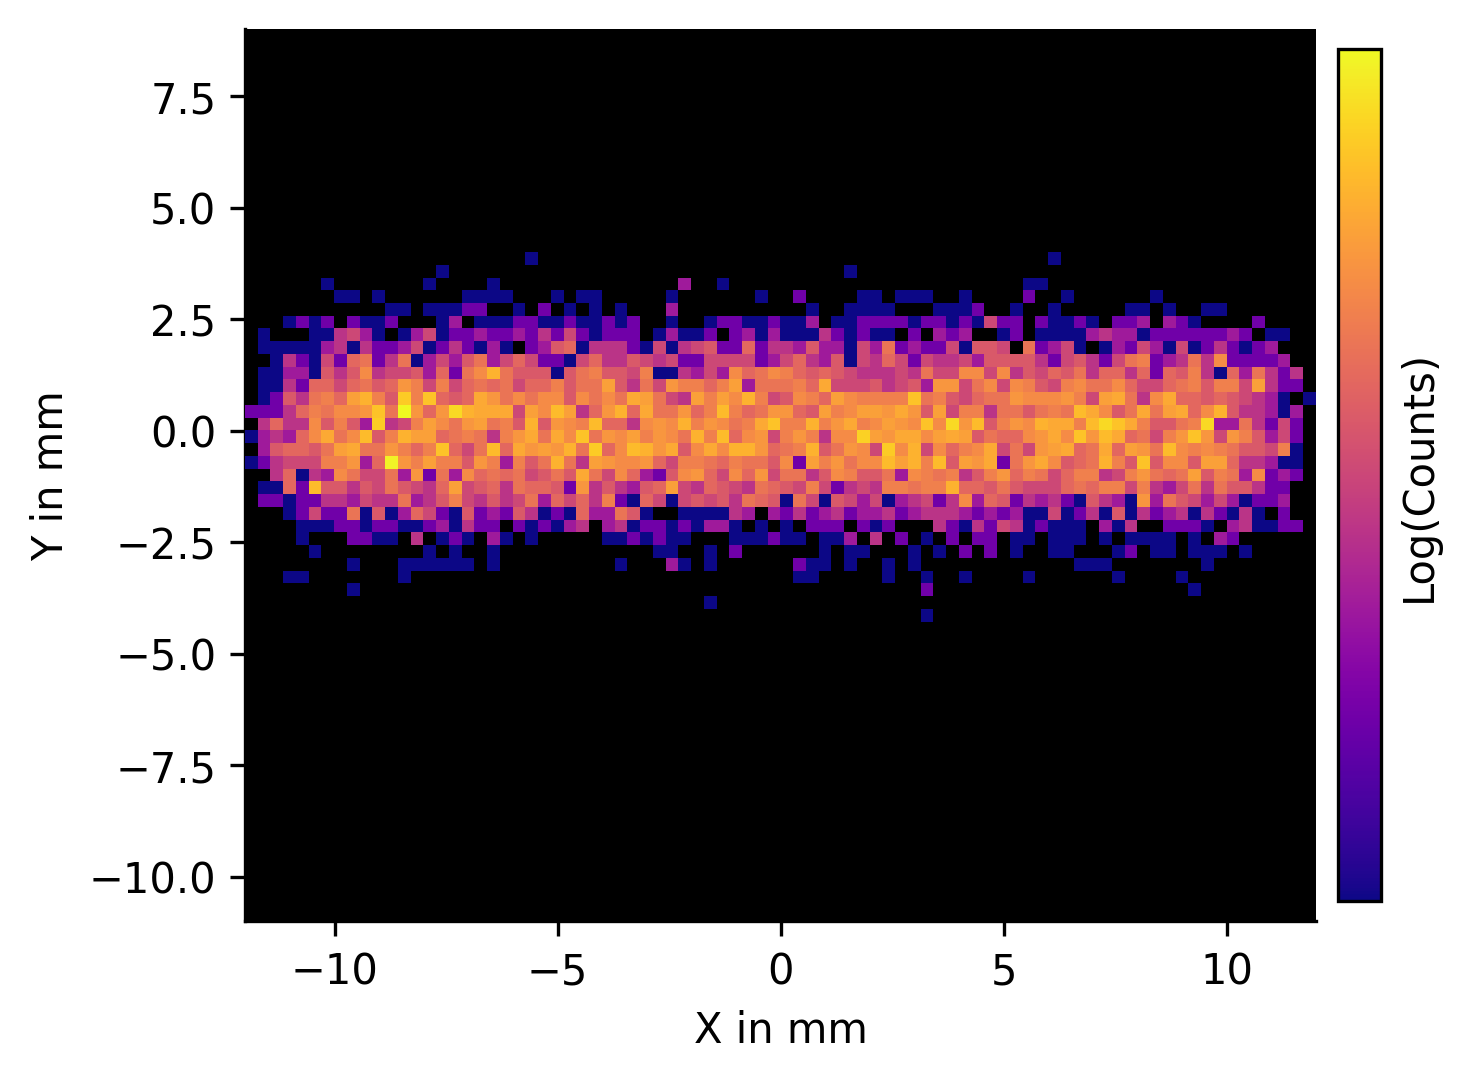
\includegraphics[width=1\textwidth]{Sim_Positions.png}
        \caption{Ionen bei 1/25 eV kinetischer Energie}
        \label{fig:sim_pos}
    \end{subfigure}%
    \hfill
    \begin{subfigure}{.45\textwidth}
        \centering
        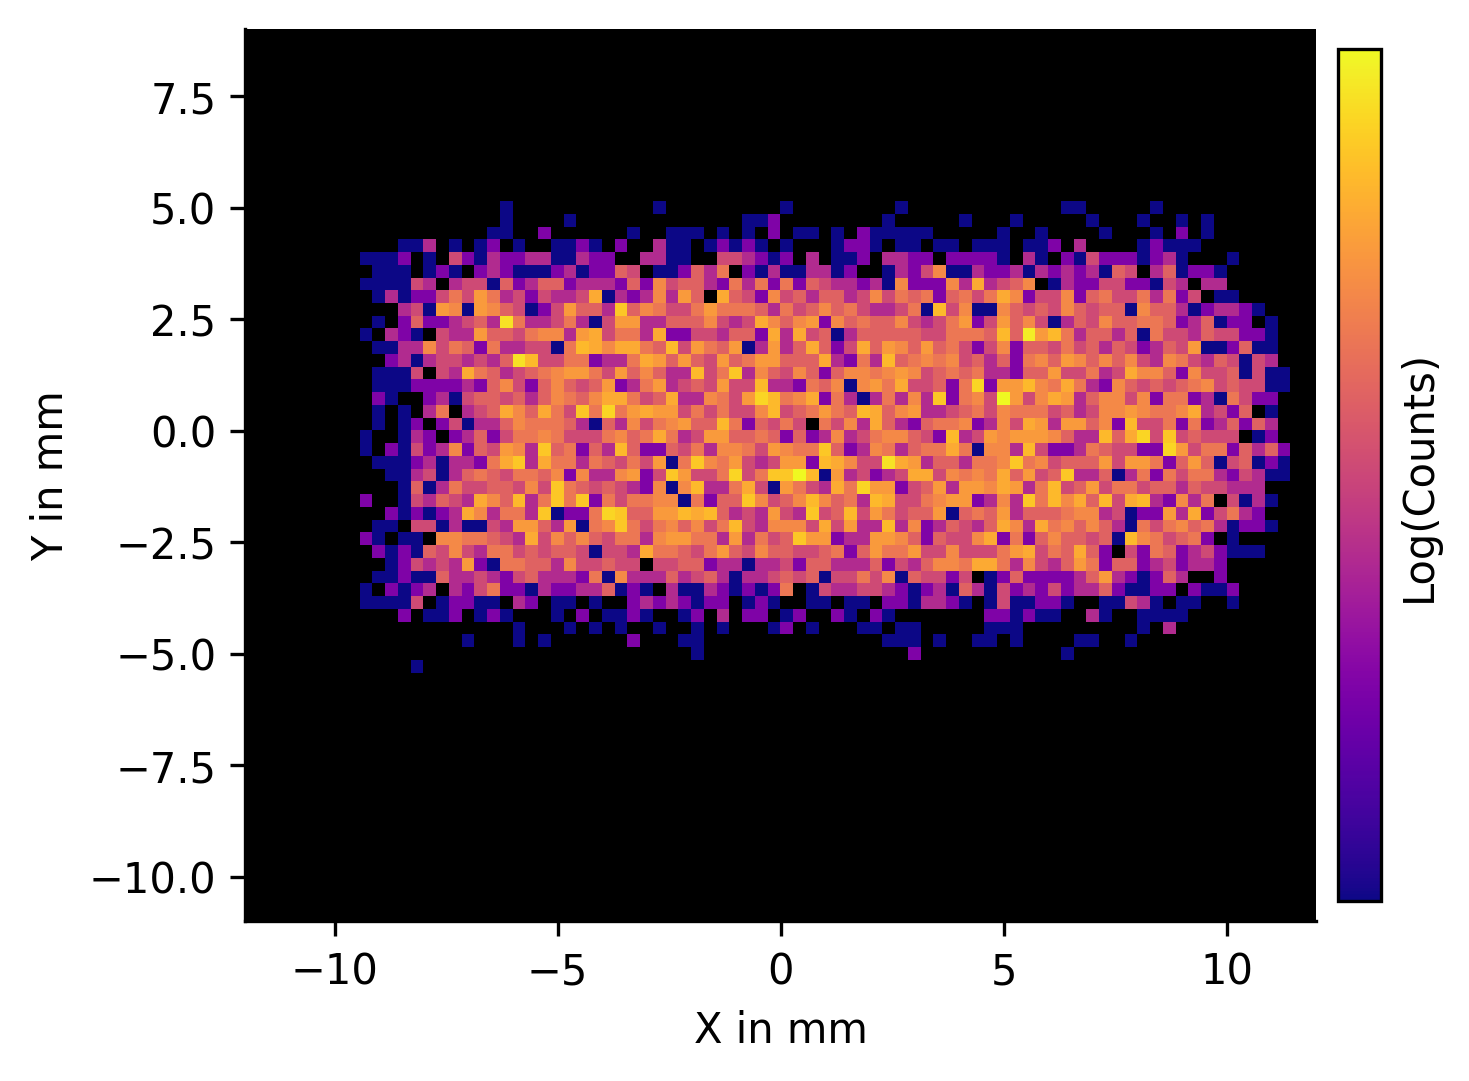
\includegraphics[width=1\linewidth]{Sim_Positions_Kinetic.png}
        \caption{Ionen bei 1/5 eV kinetischer Energie}
        \label{fig:sim_pos_kinetic}
    \end{subfigure}
    \caption[Simuliertes Abbild des Strahls auf dem Detektor bei verschiedenen Energien]{Logarithmisches Abbild des simulierten Strahls auf dem Detektor bei unterschiedlichen kinetischen Energien. Die Länge des tatsächlichen Strahls ist als Vergleich eingezeichnet. Die Bilder sind deutlich weniger gesättigt, da nicht annähernd so viele Ionen simuliert wurden, wie im Experiment über einen längeren Zeitraum gesammelt wurden. Einen Hintergrund wie im Experiment gibt es in der Simulation nicht.}
    \label{fig:sim_pos_both}
\end{figure}

Anhand dieser Vergleiche kann bereits festgestellt werden, dass die Simulation der Ionenoptik in \textit{SIMION} eine gute Übereinstimmung mit den experimentellen Daten zeigt, auch wenn nicht alle Phänomene abgebildet werden können. Die Simulation kann also genutzt werden, um die Ionenoptik des Massenspektrometers zu untersuchen und Optimierungsansätze zu finden.


\section{Untersuchung der Ionenoptik}

\subsection{Einfluss der Flugstrecke}
\subsection{Untersuchung zur Energie-Flugzeit-Korrelation}
\label{sec:delay}
\subsection{Auflösungsvermögen}

\section{Zusammenfassung und Ausblick}